\section{Digit-by Accuracy}
\begin{figure}[htb!]
    \centering
    \begin{subfigure}[b]{\textwidth}
        \centering
        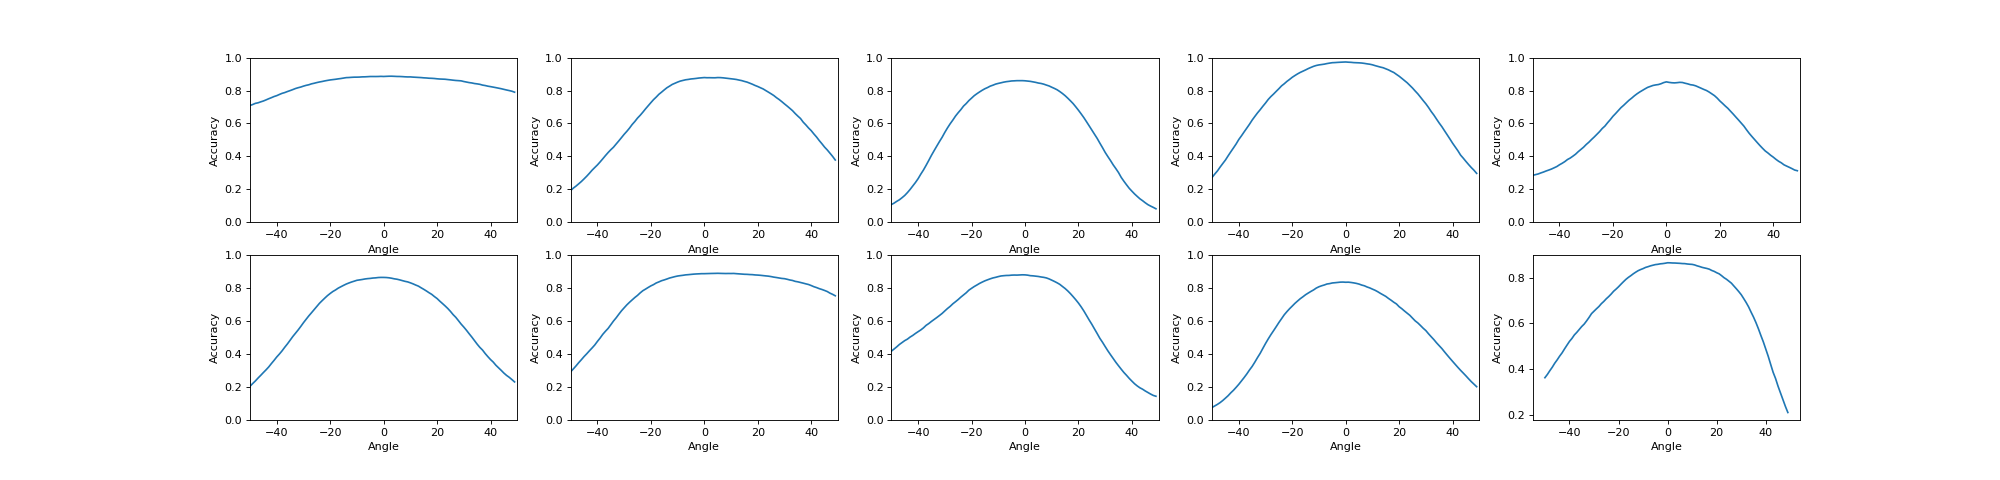
\includegraphics[width=\textwidth]{chapters/results/CNN/Rotate/accAll.png}
        \caption{Rotate}
        \label{fig:Rotate-misclass0}
    \end{subfigure}
    \begin{subfigure}[b]{\textwidth}
        \centering
        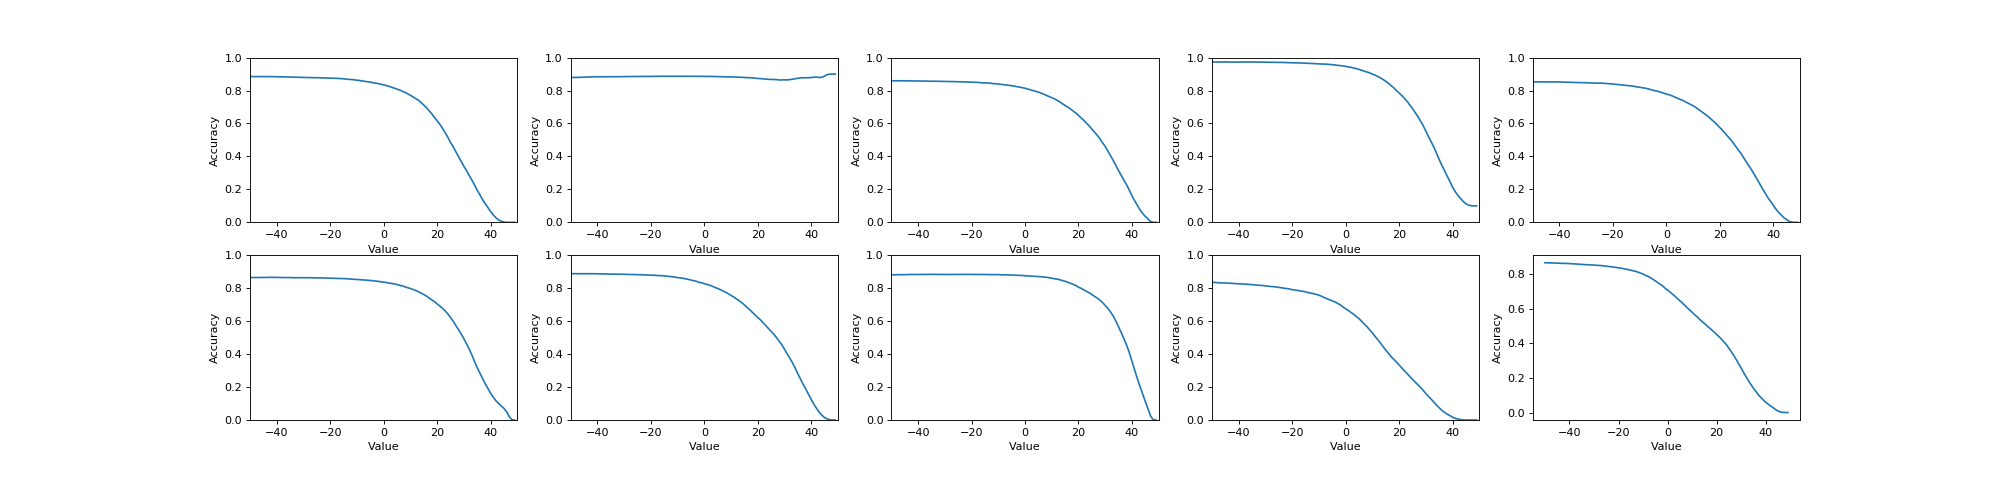
\includegraphics[width=\textwidth]{chapters/results/CNN/Shade/accAll.png}
        \caption{Shading}
        \label{fig:Rotate-misclass1}
    \end{subfigure}
    \begin{subfigure}[b]{\textwidth}
        \centering
        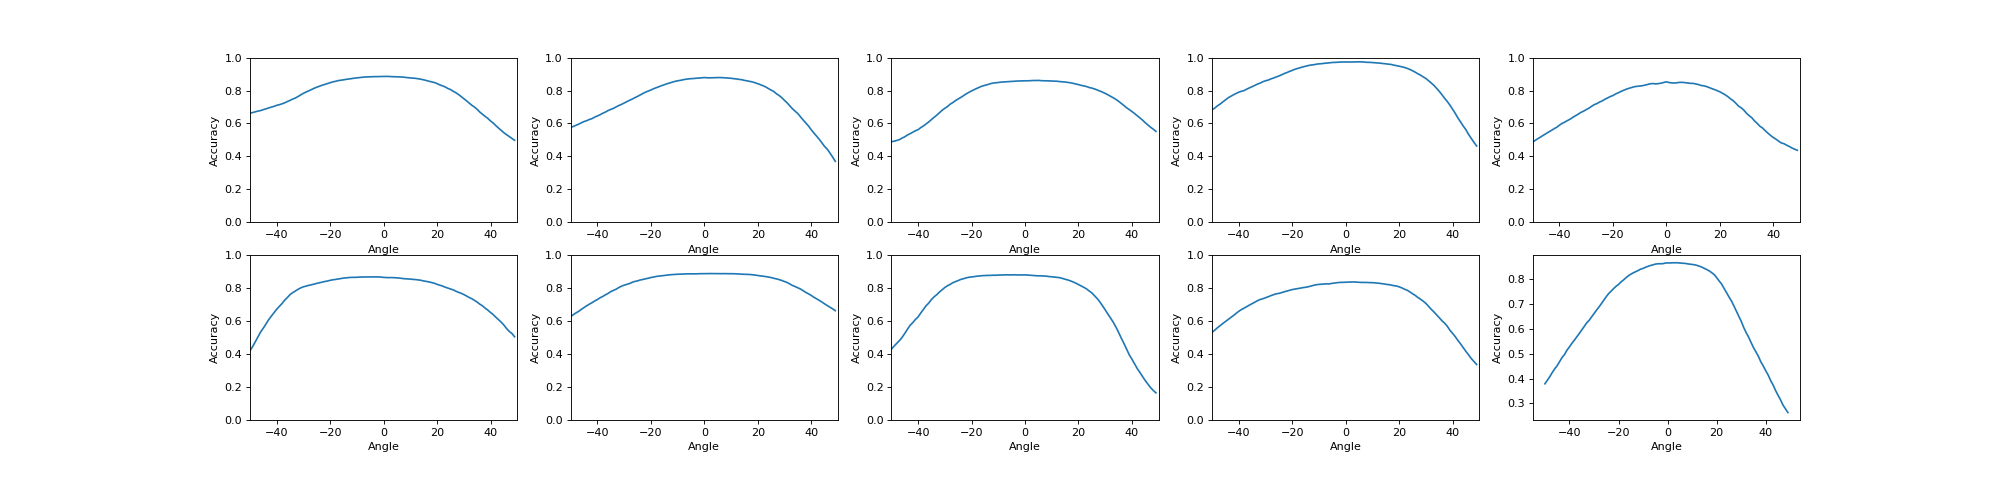
\includegraphics[width=\textwidth]{chapters/results/CNN/Shear/accAll.png}
        \caption{Shear}
        \label{fig:Rotate-misclass0}
    \end{subfigure}
    \begin{subfigure}[b]{\textwidth}
        \centering
        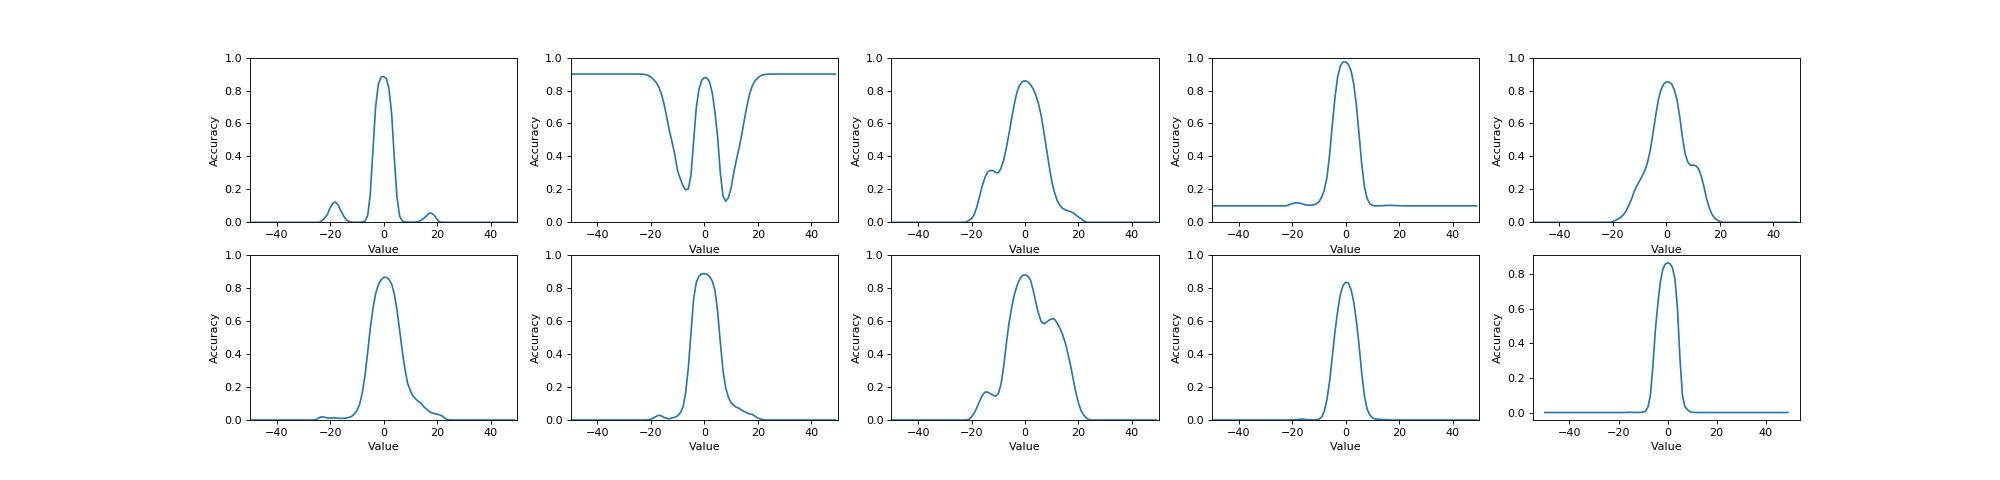
\includegraphics[width=\textwidth]{chapters/results/CNN/ShiftX/accAll.png}
        \caption{Shifting in X-axis}
        \label{fig:Rotate-misclass0}
    \end{subfigure}
    \label{fig:Rotate-misclassifications}
\end{figure}

\begin{figure}
    \centering
        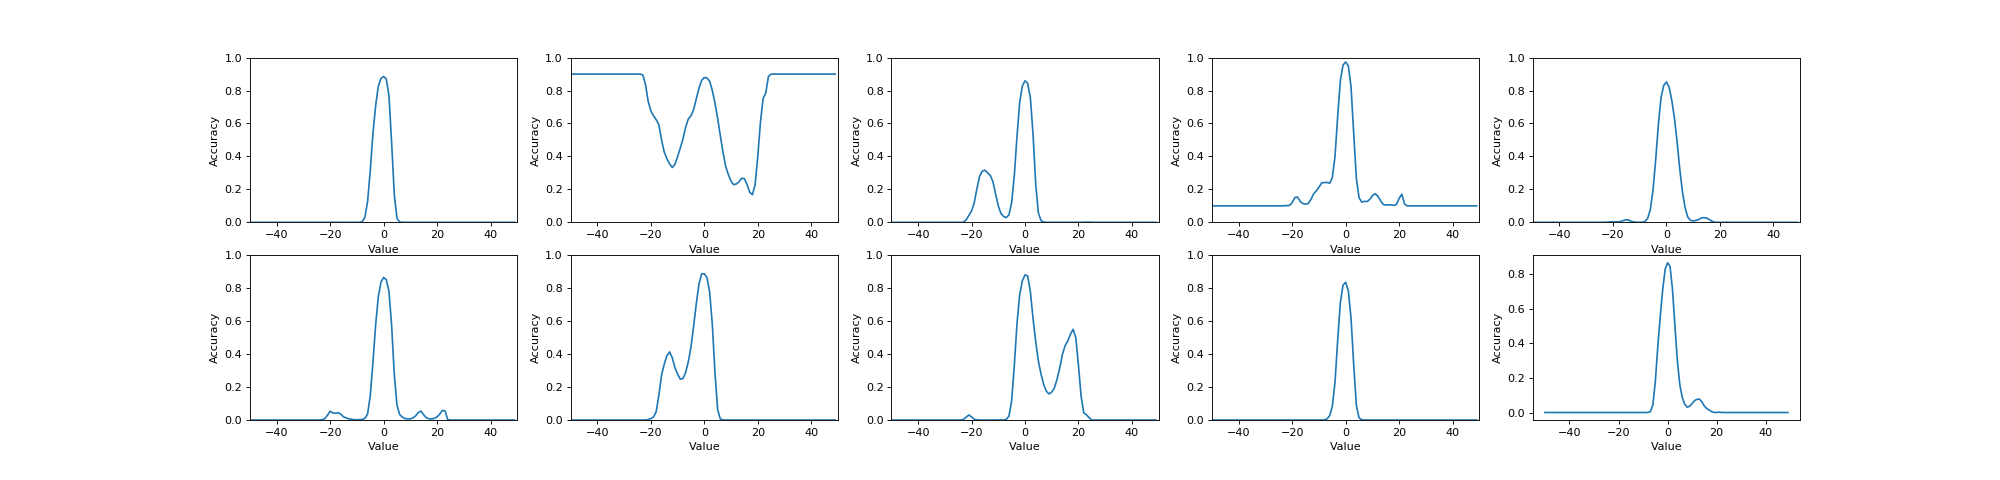
\includegraphics[width=\textwidth]{chapters/results/CNN/ShiftY/accAll.png}
        \caption{Shifting in Y-axis}
        \label{fig:Rotate-misclass0}
\end{figure}
Rotation
1.  The graph is bell shaped
2. 0 is not affected due to rotation